\subsection{The \texttt{c3} (\texttt{ret}) assembly instruction}

Assuming the x86 instruction set, \code{ret} does two things:

\begin{enumerate}
  \item Pops a memory address off the stack
  \item Jumps to that memory address
\end{enumerate}

What the CPU does in order to achieve the above is:

\begin{enumerate}
  \item Set the instruction pointer, which is stored in register \texttt{\%eip}\footnote{Source: Control Flow Instructions, \url{https://flint.cs.yale.edu/cs421/papers/x86-asm/asm.html}}, to the value on top of the stack (at the address pointed to by register \texttt{\%rsp}).
  \item Decrease the stack pointer (in register \texttt{\%rsp}) with the address size (32 bits or 64 bits depending on architecture).
\end{enumerate}

I've illustrated this in an example on \autoref{fig:ret}:

\begin{figure}[H]
  \centering
  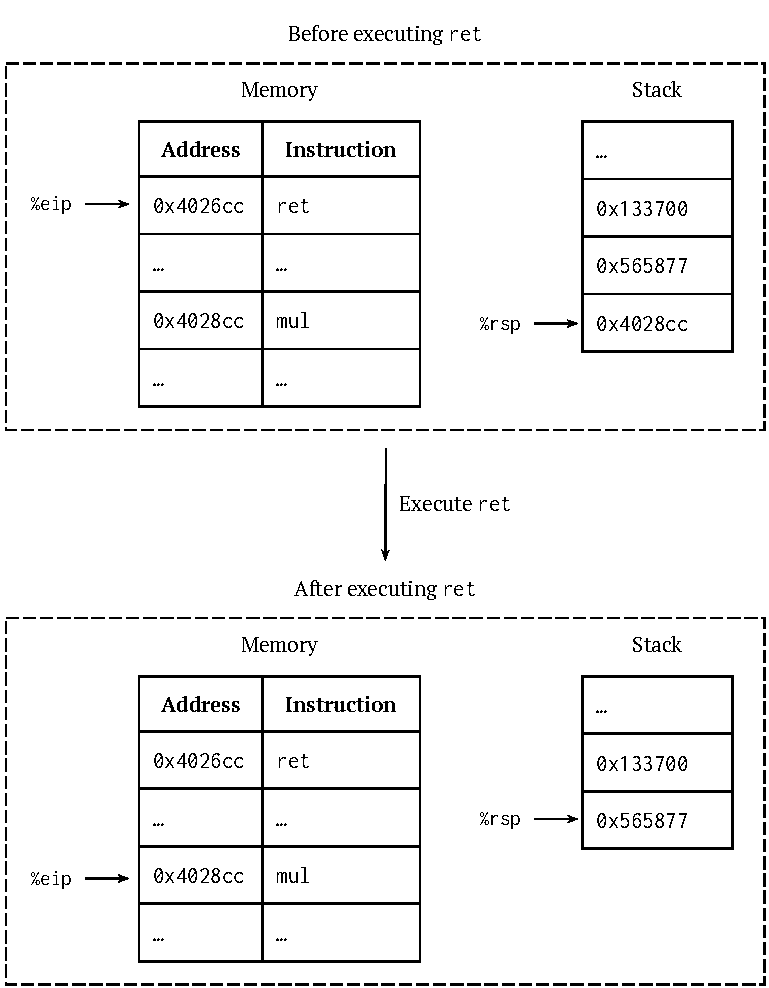
\includegraphics{figures/ret-example.pdf}
  \caption{An illustration of how the \code{ret} instruction manipulates registers in the CPU when executing the \code{ret} instruction. Before executing \code{ret}, the value \code{0x4028cc} is on top of the stack. After execution, the stack has been popped and the instruction pointer points to \code{0x4028cc}.}
  \label{fig:ret}
\end{figure}
